\documentclass[12pt, a4paper]{article} % book, report, article, letter, slides
                                       % letterpaper/a4paper, 10pt/11pt/12pt, twocolumn/twoside/landscape/draft

%%%%%%%%%%%%%%%% PACKAGES %%%%%%%%%%%%%%%%%%%%%

\usepackage[utf8]{inputenc} % encoding

\usepackage[english]{babel} % use special characters and also translates some elements within the document.

\usepackage{amsmath}        % Math
\usepackage{amsthm}         % Math, \newtheorem, \proof, etc
\usepackage{amssymb}        % Math, extended collection
\usepackage{bm}             % $\bm{D + C}$
\newtheorem{theorem}{Theorem}[section]     % \begin{theorem}\label{t:label}  \end{theorem}<Paste>
\newtheorem{corollary}{Corollary}[theorem]
\newtheorem{lemma}[theorem]{Lemma}
\newenvironment{claim}[1]{\par\noindent\underline{Claim:}\space#1}{}
\newenvironment{claimproof}[1]{\par\noindent\underline{Proof:}\space#1}{\hfill $\blacksquare$}

\usepackage{hyperref}       % Hyperlinks \url{url} or \href{url}{name}

\usepackage{parskip}        % \par starts on left (not idented)

\usepackage{abstract}       % Abstract

\usepackage{tocbibind}      % Adds the bibliography to the table of contents (automatically)

\usepackage{graphicx}       % Images
\graphicspath{ {./images/} }

\usepackage[vlined,ruled]{algorithm2e} % pseudo-code

% \usepackage[document]{ragged2e}  % Left-aligned (whole document)
% \begin{...} ... \end{...}   flushleft, flushright, center

%%%%%%%%%%%%%%%% CODE %%%%%%%%%%%%%%%%%%%%%

\usepackage{minted}         % Code listing
% \mint{html}|<h2>Something <b>here</b></h2>|
% \inputminted{octave}{BitXorMatrix.m}

%\begin{listing}[H]
  %\begin{minted}[xleftmargin=20pt,linenos,bgcolor=codegray]{haskell}
  %\end{minted}
  %\caption{Example of a listing.}
  %\label{lst:example} % You can reference it by \ref{lst:example}
%\end{listing}

\newcommand{\code}[1]{\texttt{#1}} % Define \code{foo.hs} environment

%%%%%%%%%%%%%%%% COLOURS %%%%%%%%%%%%%%%%%%%%%

\usepackage{xcolor}         % Colours \definecolor, \color{codegray}
\definecolor{codegray}{rgb}{0.9, 0.9, 0.9}
% \color{codegray} ... ...
% \textcolor{red}{easily}

%%%%%%%%%%%%%%%% CONFIG %%%%%%%%%%%%%%%%%%%%%

\renewcommand{\absnamepos}{flushleft}
\setlength{\absleftindent}{0pt}
\setlength{\absrightindent}{0pt}

%%%%%%%%%%%%%%%% GLOSSARIES %%%%%%%%%%%%%%%%%%%%%

%\usepackage{glossaries}

%\makeglossaries % before entries

%\newglossaryentry{latex}{
    %name=latex,
    %description={Is a mark up language specially suited
    %for scientific documents}
%}

% Referene to a glossary \gls{latex}
% Print glossaries \printglossaries

\usepackage[acronym]{glossaries} %

% \acrshort{name}
% \acrfull{name}
\newacronym{kcol}{$k$-COL}{$k$-coloring problem}
\newacronym{scol}{SEARCH-$k$-COL}{Search $k$-coloring problem}
\newacronym{2col}{$2$-COL}{$2$-coloring problem}
\newacronym{e2sat}{$E2$-SAT}{Exactly 2-SAT}

%%%%%%%%%%%%%%%% HEADER %%%%%%%%%%%%%%%%%%%%%

\usepackage{fancyhdr}
\pagestyle{fancy}
\fancyhf{}
\rhead{TODO}
\lhead{TODO}
\rfoot{Page \thepage}

%%%%%%%%%%%%%%%% TITLE %%%%%%%%%%%%%%%%%%%%%

\title{%
  TODO
}
\author{%
  Arnau Abella \\
  \large{Universitat Polit\`ecnica de Catalunya}
}
\date{\today}

%%%%%%%%%%%%%%%% DOCUMENT %%%%%%%%%%%%%%%%%%%%%

\begin{document}

\maketitle

\tableofcontents

\begin{abstract}
\noindent
  TODO
\end{abstract}


\section{a}\label{a}

\subsection{b}\label{b}

\subsubsection{c}\label{c}

\begin{algorithm}[H]
  \SetAlgoNoLine
  \SetKwInOut{Input}{Input}
  \SetKwInOut{Output}{Output}
  \Input{Given the graph $G = \langle V, E \rangle$ and $k$ colors.}
  \Output{A solution $a := a_1,\dots,a_{|V|}$ of \acrshort{scol}, $a_i = \{1..k\}$ \\ or $UNSAT$.}
  \BlankLine
  \For(\tcp*[f]{$|V|$ times}){$i \leftarrow 1$ \KwTo $|V|$}{
    \For(\tcp*[f]{$|K|$ times}){$j \leftarrow 1$ \KwTo $|k|$}{
      \tcp{Each assignment is a copy of the vector $a$}
      \tcp{At most $|v|^{|k|}$ copies}
      $a := (a_1,\dots,a_{i-1}, a_i = j)$;
    }
    \If{$i = |V|$}{
      Test if $x := (x_1 = a_1, \dots, x_n = a_{|V|})$ is a valid assignment using \acrshort{kcol}; \tcp{p(n)-time}
      If it is a valid assignment, then \emph{halt} and return $a$;
     }
  }
  return $UNSAT$;
  \caption{Na\"ive \acrshort{scol} Algorithm}
  \label{scol}
\end{algorithm}

\newpage

Na\"ive. $\hat{y} = x + 1$

This is a bibliography cite\cite{einstein}.

{\tiny Large}
{\scriptsize Large}
{\footnotesize Large}
{\small Large}
{\large \textrm{Very descriptive text.}}
{\large \textsf{Very descriptive text.}}
{\large \texttt{Very descriptive text.}}

This is a footnote\footnote{my first footnote}.

\begin{figure}[h]
  \centering
  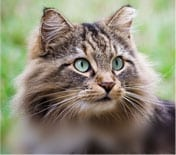
\includegraphics[scale=0.5]{cat}  % [width=\textwidth, height=4cm],
  \caption{Example of a cat}
  \label{fig:cat}
\end{figure}

This is a very cute cat, figure \ref{fig:cat}

\begin{table}
\begin{center}
\begin{tabular}{ |c|c|c| }
 \hline
 cell1 & cell2 & cell3 \\
 cell4 & cell5 & cell6 \\
 cell7 & cell8 & cell9 \\
 \hline
\end{tabular}
\end{center}
\caption{Table to test captions and labels}
\label{table:1}
\end{table}

%%%%%%%%%%%%%%%% BIBLIOGRAPHY %%%%%%%%%%%%%%%%%%%%%

\bibliographystyle{unsrt} % abbrv, aplha, plain, abstract, apa, unsrt,
\bibliography{refs}

\end{document}
